\graphicspath{{chapters/images/0201/}}

\chapter{What is statistical learning?}
  
  \section{Definition of statistical learning}
    In general, a statistical learning problem can be formalized as follows:

    \begin{itemize}
      \item $Y$ : response/dependent/outcome variable
      \item $\vec{X} = (X_1, \dots, X_p)$: vector of predictors/features/independent variables/covariates
    \end{itemize}
    We assume that there is a relationship between $Y$ and $\vec{X}$, which can be written as:

    $$Y = f(\vec{X}) + \varepsilon $$
    Where:
    \begin{itemize}
      \item $f(\vec{X})$ is the deterministic (but unknown) function of the vector $\vec{X} = (X_1, \dots, X_p)$
      \item $\varepsilon$ is the error (stochastic part), for which we assume the following properties:
      \begin{itemize}
        \item[$\bullet$] $E[\varepsilon] = 0$ (Its expected value is zero)
        \item[$\bullet$] $\varepsilon \perp \vec{X}$ (It is independent from $\vec{X}$)
      \end{itemize}
    \end{itemize}
    Therefore, the expression \textbf{statistical learning} encompasses different methods to estimate $f(\vec{X})$. 

  \section{Why estimate \textit{f}?}
    There are two main reasons to estimate $f$, those two being \textbf{prediction} and \textbf{inference}.
  
    \subsection{Prediction}
      Predict $Y$ when we only have observations about $\vec{X}$. Since $E[\varepsilon] = 0$, we usually take:

      $$\hat{Y} = \hat{f} (\vec{X})$$

      With $\hat{f}$ being our estimate of $f$.
      
      If this is the only reason to estimate $f$, then $\hat{f}$ can be a black-box method (deep learning).
      The accuracy of $\hat{Y}$ as a predictor of $Y$ can be described calculating the expected \textbf{MSE}, the test Mean Squared Error %TODO ref image:

      \begin{align*}
        E[(Y&-\hat{f}(\vec{X}))^2 \,|\, \vec{X} = \vec{x}\,] = 
        & \text{where } \hat{f} \text{ is a fixed known function}\\
        & = E[(f(\vec{X}) + \varepsilon - \hat{f}(\vec{X}))^2]
        & \text{since } Y = f(\vec{X}) + \varepsilon \\
        & = E[(f(\vec{X}) - \hat{f}(\vec{X})) + \varepsilon)^2]
        & \text{rearranging} \\
        & = E[(f(\vec{X}) - \hat{f}(\vec{X}))^2 + \varepsilon^2 + 2\varepsilon(f(\vec{X}) - \hat{f}(\vec{X}))]
        & \text{solving the square} \\
        & = E[(f(\vec{X}) - \hat{f}(\vec{X}))^2] + E[\varepsilon^2] + 2E[\varepsilon(f(\vec{X}) - \hat{f}(\vec{X}))]
        & \text{separating the expectations}
      \end{align*}
      
      Furthermore, since we know that:
      \begin{align*}
        Var(\varepsilon) 
        & = E[(\varepsilon - E(\varepsilon))^2]
        & \text{formal definition of variance} \\
        & = E[\varepsilon^2] - (E[\varepsilon])^2  
        & \text{definition generally used during calculation} \\
        & = E[\varepsilon^2] 
        & \text{since } E[\varepsilon] = 0 \\
      \end{align*}

      Thus we get:
      \begin{align*}
        E[(Y&-\hat{f}(\vec{X}))^2 \,|\, \vec{X} = \vec{x}\,] = \\
        & = E[(f(\vec{X}) - \hat{f}(\vec{X}))^2] + Var(\varepsilon) + 2E[\varepsilon(f(\vec{X}) - \hat{f}(\vec{X}))]
        & \text{substituting } E[\varepsilon^2] = Var(\varepsilon) \\
        & = (f(\vec{X}) - \hat{f}(\vec{X}))^2 + Var(\varepsilon) + 2(f(\vec{X}) - \hat{f}(\vec{X}))E[\varepsilon]
        & \text{since } f(\vec{X}) - \hat{f}(\vec{X}) \text{ is a constant}\\
        & = (f(\vec{X}) - \hat{f}(\vec{X}))^2 + Var(\varepsilon)
        & \text{since } E[\varepsilon] = 0 \\
      \end{align*}

      With:
      \begin{itemize}
        \item $(f(\vec{X}) - \hat{f}(\vec{X}))^2$ being the \textbf{reducible error}. The model choice can increase or reduce this value, hence it is mostly controllable.
        \item $Var(\varepsilon)$ being the \textbf{irreducible error}. This value depends on the innate randomness present in the data, hence you can only try and minimize it by deciding which variables to use in your prediction (but it will never be zero otherwise you would have a deterministic situation).
      \end{itemize}

      % TODO Add image of graph

    \subsection{Inference}
      Inference is used when you want to understand the relation between $Y$ and $\vec{X}$ (and not just be able to make predictions). Namely, inference answers questions such as:
      \begin{itemize}
        \item Which predictors/factors are most associated with the response?
        \item What is the relationship between $Y$ and $X_j$?
      \end{itemize}

  \section{How to extimate \textit{f}?}
    Given some \textbf{training data} $(\vec{x}_i, y_i), \, i = 1, \dots, n$, where $\vec{x}_i = (x_{i1}, \dots, x_{ip})^t$ is the vector of observations of unit $i$ while $y_i$ is the response for unit $i$, broadly speaking there are two types of methods to estimate $f$: \textbf{parametric methods} and \textbf{non-parametric methods}.

    \subsection{Parametric methods}
      In order to use parametric methods, we make an assumption about the functional form of $f(\vec{X})$, that assumption being that the form of the function depends on some parameters (which we can estimate). An example of parametric method is \textbf{linear regression}, which implies that $f(\vec{X})$ is in the form:

      $$f(\vec{X}) = \beta_0 + \beta_1 X_1 + \beta_2 X_2 + \dots + \beta_p X_p$$

      Given this assumption, statistical learning becomes \textbf{fitting} (or training) the model on the data, which means estimating the parameters $\hat{\beta_0}, \hat{\beta_1}, \dots, \hat{\beta_p}$ such that:

      $$\hat{f}(\vec{X}) = \hat{\beta_0} + \hat{\beta_1} X_1 + \hat{\beta_2} X_2 + \dots + \hat{\beta_p} X_p$$

      The main disadvantage of these methods is that they may be \textbf{too restrictive}.

      Notice that linear models are \underline{linear in the parameters}, not in the predictors, hence:
      \begin{itemize}
        \item $f(X_1) = \beta_0 + \beta_1 X_1 + \beta_2 X_1^2 + \beta_3 X_1^3 + \varepsilon$ (polynomial regression) is a linear model.
        \item $f(X_1) = \beta_0 X_1^{\beta_1}$ is \underline{not} a linear model.
      \end{itemize}

    \subsection{Non-parametric methods}
      Non-parametric methods do not make any explicit assumption on the function form of $f(\vec{X})$. These methods want to estimate $f$ by getting as close as possible to the data, without being too \textit{rough or wiggly} (basically \textbf{overfitting}).

    \subsection{Parametric vs non-parametric methods}
      Despite parametric methods being more restrictive than non-parametric ones, we might still choose to adopt the former for the sake of interpretability and generalizability outside of the training data. %TODO sezione ampliabile

  \section{Bias-variance trade-off}

    Assume you have some data pairs in the form $(x_i, y_i), \, i = 1, \dots, n$; you can then define the estimate function $\hat{f}(x)$ as a linear model with up to $n-1$ parameters (more parameters give the same result as $n-1$ parameters) and an intercept value. You could thus use, for instance, the models:
    \begin{align*}
      & 1 \text{ parameter}    &f(x) &= \beta_0 + \beta_1x + \varepsilon \\
      & 2 \text{ parameters}   &f(x) &= \beta_0 + \beta_1x + \beta_2x^2 + \varepsilon \\
      & \vdots                 &     &\vdots \\
      & n-1 \text{ parameters} &f(x) &= \beta_0 + \beta_1x + \beta_2x^2 + \dots + \beta_{n-1}x^{n-1} + \varepsilon \\
    \end{align*}
    You could choose the model with the highest number of parameters; this model would explain all the variance of the training data ($R^2=1$) yet it would be very complex and perform badly with new data points. On the other hand a model with a lower number of parameters would explain less of the variance of the training data, yet it could perform better with new data points.

    % TODO Add image of bias graph

    Keeping in mind that $Y$ is random and that $\hat{f}$ is a random variable estimated from the data,
    when using the general formula to determine how well a model performs at generic $\vec{X}$, we notice:
    \begin{align*}
      E[(Y&-\hat{f}(\vec{X}))^2 \,|\, \vec{X} = \vec{x}\,] = \\
      & = E[(f(\vec{X}) + \varepsilon - \hat{f}(\vec{X}))^2] 
      & \text{since } Y = f(\vec{X}) + \varepsilon \\
      & = E[(f(\vec{X}) + \varepsilon - \hat{f}(\vec{X}) + E[\hat{f}(\vec{X})] - E[\hat{f}(\vec{X})])^2]
      & \text{since } E[\hat{f}(\vec{X})] - E[\hat{f}(\vec{X})] = 0\\
      & = E[((f(\vec{X}) - E[\hat{f}(\vec{X})])+ \varepsilon + (E[\hat{f}(\vec{X})] - \hat{f}(\vec{X})))^2]
      & \text{grouping}\\
      & = E[(f(\vec{X}) - E[\hat{f}(\vec{X})])^2] + E[\varepsilon^2] + E[(E[\hat{f}(\vec{X})] - \hat{f}(\vec{X}))^2] \, +
      & \\
      & \;\;\;\, + 2E[(f(\vec{X}) - E[\hat{f}(\vec{X})])\,\varepsilon] \, + & \\
      & \;\;\;\, + 2E[(f(\vec{X}) - E[\hat{f}(\vec{X})])(E[\hat{f}(\vec{X})] - \hat{f}(\vec{X}))] \, + 
      & \text{solving the square and}\\
      & \;\;\;\, + 2E[(E[\hat{f}(\vec{X})] - \hat{f}(\vec{X}))\,\varepsilon] \,
      & \text{dividing the expectations}\\
    \end{align*}

    But notice that:
    \begin{align*}
      E[(f(\vec{X}) - E[\hat{f}(\vec{X})])\,\varepsilon] 
      & = E[\varepsilon](f(\vec{X}) - E[\hat{f}(\vec{X})]) 
      & \text{since } f(\vec{X}) - E[\hat{f}(\vec{X})] \text{ is constant}\\
      & = 0
      & \text{since } E[\varepsilon] = 0 \\
    \end{align*}
    \begin{align*}
      E[(f(\vec{X}) & - E[\hat{f}(\vec{X})])(E[\hat{f}(\vec{X})] - \hat{f}(\vec{X}))] = \\
                    & = (f(\vec{X}) - E[\hat{f}(\vec{X})])E[E[\hat{f}(\vec{X})] - \hat{f}(\vec{X})]
                    & \text{since } f(\vec{X}) - E[\hat{f}(\vec{X})] \text{ is constant} \\
                    & = (f(\vec{X}) - E[\hat{f}(\vec{X})])E[ \hat{f}(\vec{X}) - \hat{f}(\vec{X})]
                    & \text{since } \hat{f}(\vec{X}) \text{ is a constant} \\
                    & = (f(\vec{X}) - E[\hat{f}(\vec{X})])E[0] \\
                    & = 0
    \end{align*}
    \begin{align*}
      E[(E[\hat{f}(\vec{X})] - \hat{f}(\vec{X}))\,\varepsilon]
      & = E[\varepsilon]E[E[\hat{f}(\vec{X})] - \hat{f}(\vec{X})]
      & \text{since } \varepsilon \perp \vec{X} \implies E[\varepsilon\vec{X}] = E[\varepsilon]E[\vec{X}]\\
      & = 0
      & \text{since } E[\varepsilon] = 0 \\
    \end{align*}
    
    Therefore we can simplify as:
    \begin{align*}
    E[(Y-\hat{f}(\vec{X}))^2 \,|\, \vec{X} = \vec{x}\,]
    & = E[(f(\vec{X}) - E[\hat{f}(\vec{X})])^2] &+ &E[\varepsilon^2] &+ &E[(E[\hat{f}(\vec{X})] - \hat{f}(\vec{X}))^2] \\
    & = f(\vec{X}) - E[\hat{f}(\vec{X})])^2 &+ &Var(\varepsilon) &+ &Var(\hat{f}(\vec{X})) 
    \end{align*} 
    Where:
    \begin{itemize}
      \item $f(\vec{X}) - E[\hat{f}(\vec{X})])^2$ is the \textbf{bias}
      \item $Var(\varepsilon)$ is the irreducible error
      \item $Var(\hat{f}(\vec{X}))$ is the \textbf{variance} of the model
    \end{itemize}
    \textbf{Bias} refers to the error that is introduced by approximating a problem, which may be extremely complicated, by a much
    simpler model. If an estimated model performs well on the training data but it does not perform well on new data, the estimated model has high bias. If an estimated model performs well on multiple data sets, the estimated model has low bias. \textit{High bias means that an estimated model is far from the real model}. \\\\
    \textbf{Variance} refers instead to the amount by which $\hat{f}$ would change if we
    estimated it using a different training data set. Ideally, the $\hat{f}$ calculated 
    through different datasets should be not significantly different, the model should be fitted equivalently using a different training dataset. The more flexible models, the more they are influenced by a changes of the training dataset. \\
    In order to minimize the expected error, we need to achieve low bias and low variance. In practice, one needs to find a good trade-off between bias and variance, since reducing one often involves increasing the other. In general:
    \begin{itemize}
      \item A \textbf{simpe model} has high bias (it is far from the real model) and low variance (when fitting using different training data you get similar estimated parameters).
      \item A \textbf{complex model} has low bias and high variance, as the complexity of the model has the aim of making it as near as possible to the real $ f $.
    \end{itemize}
    Both in parametric and non-parametric methods, you generally have at least one \textbf{tuning parameter}, which is a parameter that can be tweaked (for instance the degree of the polinomial) in order to choose the balance between bias and variance, as it can be seen in figure \ref{MSEVarianceBias}.
   
\begin{figure}[h]
\label{MSEVarianceBias}
\caption{  
(Image of Sohil et al., 2022. As the flexibility of a model increases, the Bias decreases, and the varaiance of the model increases}
\centering
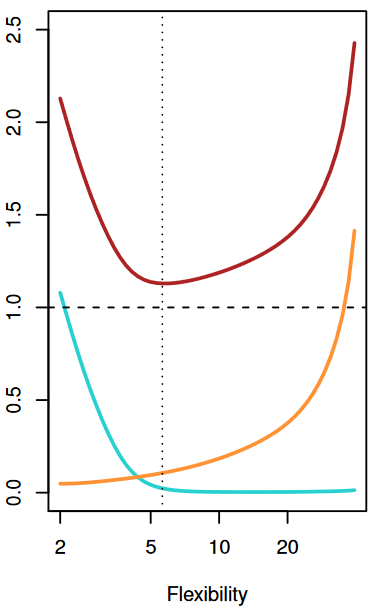
\includegraphics[width=0.3\textwidth]{MSEdependsonVarianceandBias}
\end{figure}

